\section[Desenvolvimento do Projeto]{Desenvolvimento do Projeto}

Esta seção apresenta informações relativas ao desenvolvimento do projeto: localização do código-fonte e documentação, arquitetura e tecnologias utilizadas, e protótipos de tela desenvolvidos. Toda a documentação do projeto pode ser encontrada na wiki do mesmo: \url{https://tools.ages.pucrs.br/estudify/estudify-wiki/-/wikis/home}.

\subsection{Repositório do Código Fonte do Projeto}
  Todo o código do projeto encontra-se distribuído em três repositórios:
\begin{itemize}
    \item código do \textit{frontend} web: \url{https://tools.ages.pucrs.br/estudify/frontend-web};
    \item código do \textit{frontend} \textit{mobile}: \url{https://tools.ages.pucrs.br/estudify/frontend-mobile};
    \item código do \textit{backend}: \url{https://tools.ages.pucrs.br/estudify/backend}.
\end{itemize}

\subsection{Banco de Dados Utilizado}
  O banco de dados escolhido foi o PostgreSQL, um banco de dados transacional que possui todas as propriedades ACID. Com isso, garante a segurança das transações, sejam elas concorrentes ou não, mantendo o seu estado inalterado mesmo frente a falhas, além de garantir a aplicação total das operações.

  Foi desenvolvido de maneira relacional, o que facilitou o tratamento dos relacionamentos entre as entidades da aplicação, como mostra o esquema conceitual desenvolvido, na Figura~\ref{fig:estudify-mc}.

\begin{figure}[H]
    \centering
    \small
    \caption{Modelo Conceitual Estudify}
    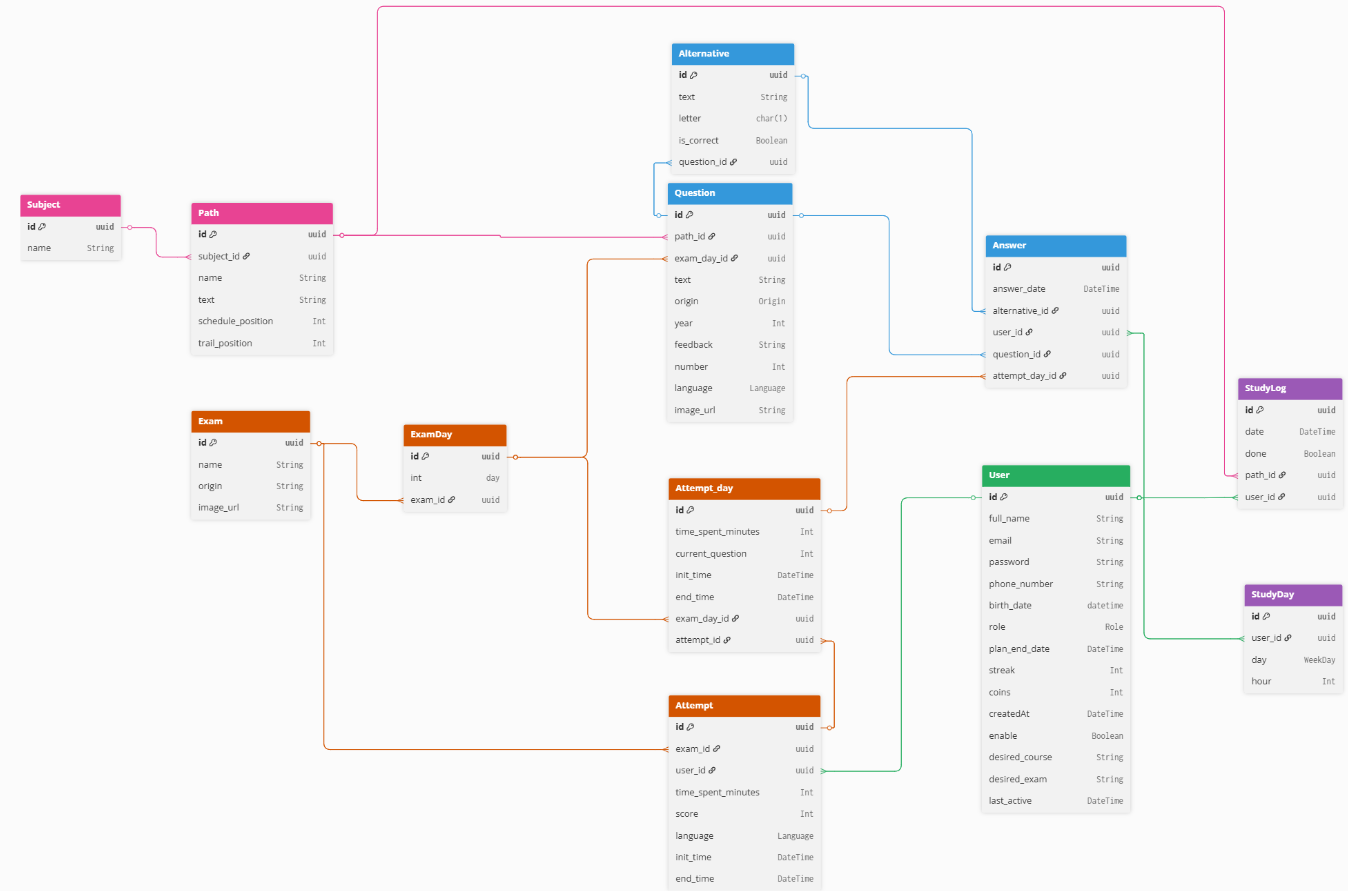
\includegraphics[width=0.9\linewidth]{conteudo/5 - ages IV/images/fig12-modelo-conceitual.png}

    Fonte: Wiki do projeto
    \label{fig:estudify-mc}
\end{figure}

\subsection{Arquitetura Utilizada}
  A arquitetura do projeto segue o padrão de Monólito Modular no \textit{back-end}, em que as funcionalidades são segregadas por domínio. Cada módulo é composto por \textit{Controllers}, responsáveis pelas rotas e requisições HTTP; \textit{Services}, que concentram as regras de negócio; \textit{Repositories}, camada isolada de comunicação com o banco de dados; e \ac{dto} (\textit{Data Transfer Objects}), que definem os contratos de entrada com validações integradas.

  A aplicação \textit{mobile} e o painel administrativo web adotam uma estrutura de pastas análoga entre si (\textit{components}, \textit{hooks}, \textit{services} e \textit{contexts}), mantendo a consistência técnica entre as frentes e permitindo que qualquer integrante do time atue em ambas.

  O fluxo de comunicação entre as camadas está ilustrado no diagrama da Figura~\ref{fig:estudify-fluxo}, evidenciando a separação entre os clientes (\textit{mobile} e web), a API e o banco de dados.

\begin{figure}[H]
    \centering
    \small
    \caption{Diagrama de fluxo da aplicação}
    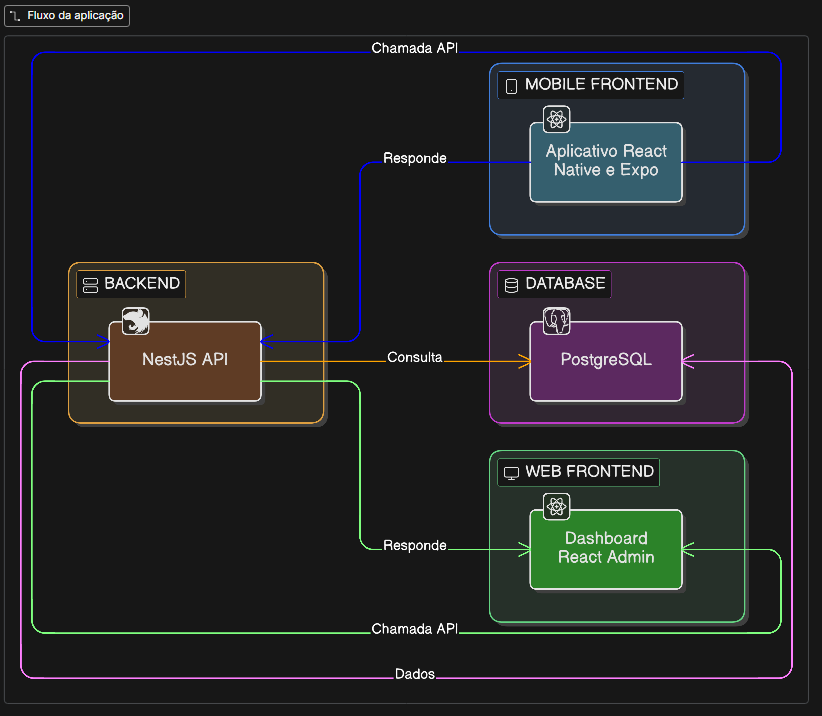
\includegraphics[width=0.9\linewidth]{conteudo/5 - ages IV/images/fig13-diagrama-fluxo.png}

    Fonte: Wiki do projeto
    \label{fig:estudify-fluxo}
\end{figure}

\subsection{Protótipos das Telas Desenvolvidas}
  Os protótipos deste projeto estão disponíveis na wiki do projeto: \url{https://tools.ages.pucrs.br/estudify/estudify-wiki/-/wikis/design}.

  A Figura~\ref{fig:estudify-prototipos} apresenta uma amostra das telas do aplicativo, contemplando os principais fluxos do usuário: o acompanhamento do progresso com os elementos de gamificação, a tela de treino com a seleção de disciplinas e tópicos, a resolução de questões e o respectivo \textit{feedback} com a explicação da resposta, além do \textit{onboarding} de primeiro acesso e da tela de perfil.

\begin{figure}[H]
    \centering
    \small
    \caption{Protótipos das telas do aplicativo \textit{mobile}}
    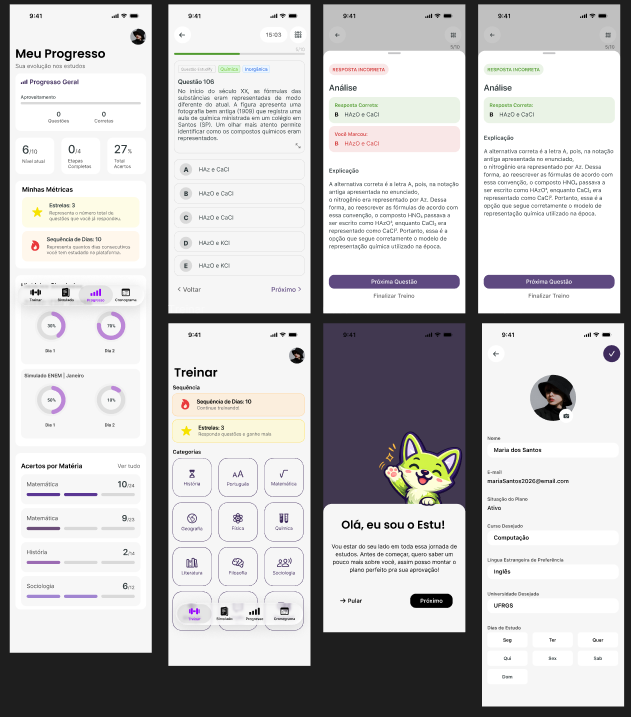
\includegraphics[width=0.9\linewidth]{conteudo/5 - ages IV/images/fig14-prototipos.png}

    Fonte: Wiki do projeto
    \label{fig:estudify-prototipos}
\end{figure}

  Além do aplicativo \textit{mobile}, o projeto conta com um painel administrativo web, destinado à gestão de conteúdo da plataforma. As Figuras \ref{fig:estudify-admin-questoes}, \ref{fig:estudify-admin-simulados} e \ref{fig:estudify-admin-importacao} apresentam as principais telas desse painel. A Figura~\ref{fig:estudify-admin-questoes} exibe a tela de gestão de questões, com busca, filtro por categoria e a listagem de todas as questões cadastradas. A Figura~\ref{fig:estudify-admin-simulados} apresenta a tela de gestão de simulados, em que é possível organizar os simulados e definir a ordem das questões que os compõem. Por fim, a Figura~\ref{fig:estudify-admin-importacao} mostra a tela de revisão das questões importadas em lote via CSV, sinalizando o \textit{status} de cada uma (sucesso, falta de imagem ou erro) para que os ajustes necessários sejam feitos antes da confirmação.

\begin{figure}[H]
    \centering
    \small
    \caption{Painel administrativo: gestão de questões}
    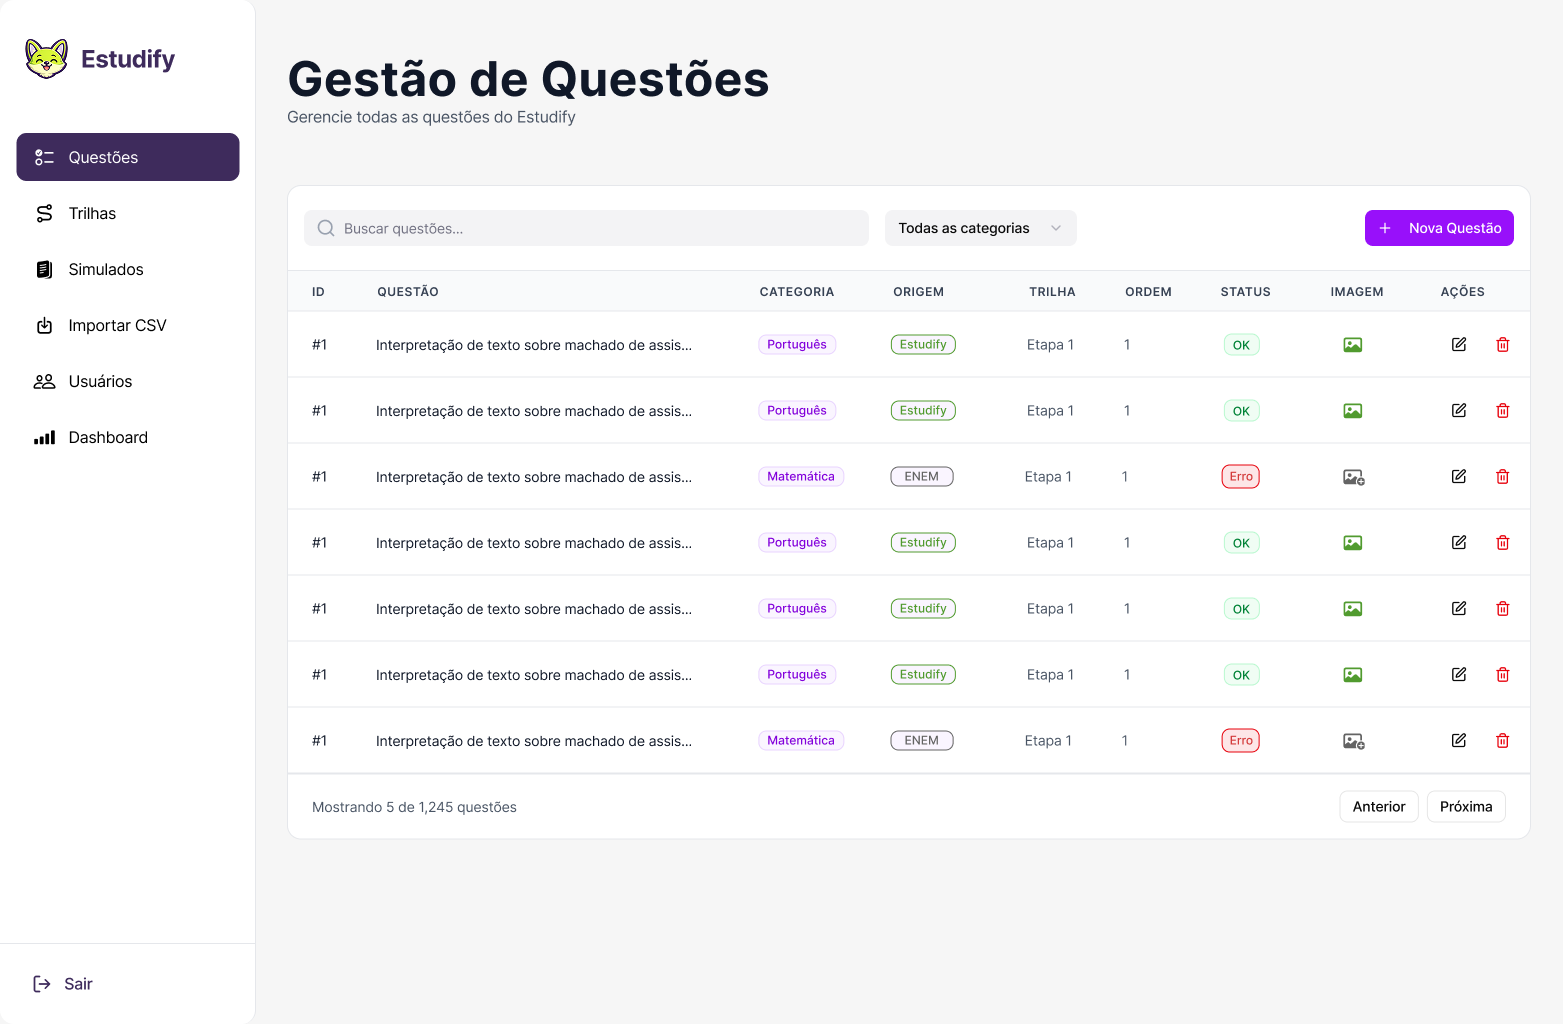
\includegraphics[width=0.7\linewidth]{conteudo/5 - ages IV/images/fig15-admin-questoes.png}

    Fonte: Wiki do projeto
    \label{fig:estudify-admin-questoes}
\end{figure}

\begin{figure}[H]
    \centering
    \small
    \caption{Painel administrativo: gestão de simulados}
    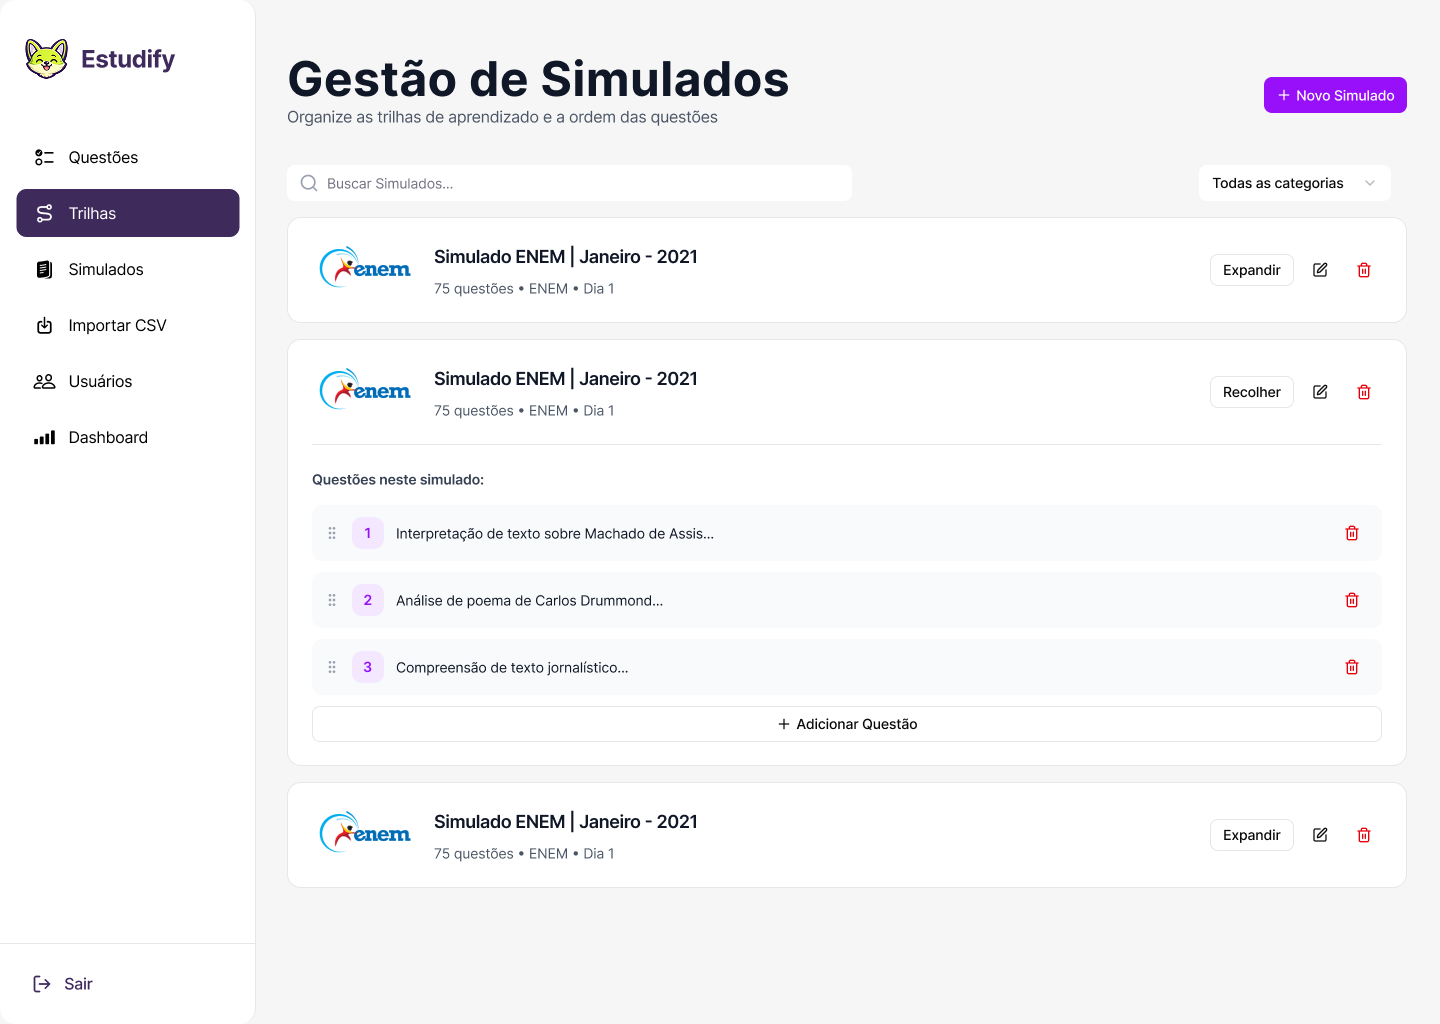
\includegraphics[width=0.7\linewidth]{conteudo/5 - ages IV/images/fig16-admin-simulados.png}

    Fonte: Wiki do projeto
    \label{fig:estudify-admin-simulados}
\end{figure}

\begin{figure}[H]
    \centering
    \small
    \caption{Painel administrativo: revisão de questões importadas via CSV}
    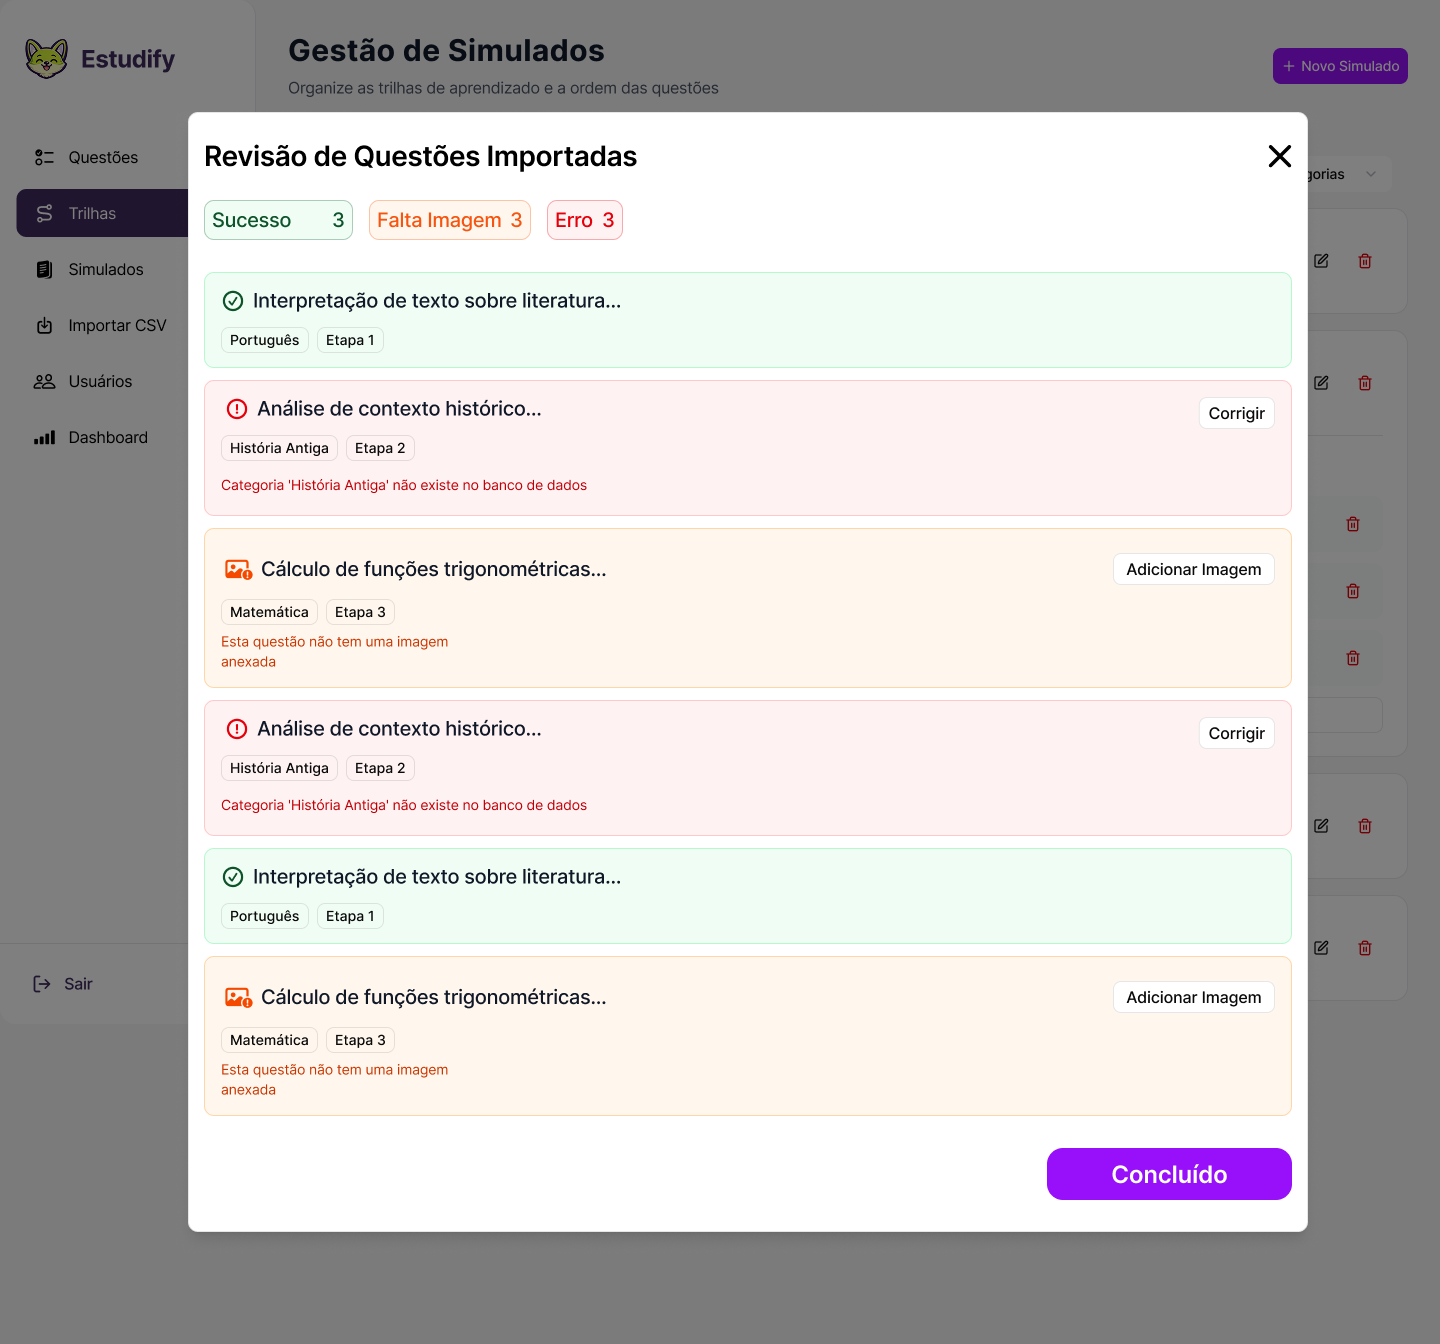
\includegraphics[width=0.55\linewidth]{conteudo/5 - ages IV/images/fig17-admin-importacao.png}

    Fonte: Wiki do projeto
    \label{fig:estudify-admin-importacao}
\end{figure}

\subsection{Tecnologias Utilizadas}
  Nesta seção serão apresentadas as principais tecnologias empregadas no desenvolvimento do projeto Estudify, destacando suas contribuições para o sucesso da implementação. As ferramentas estão organizadas conforme a camada da aplicação em que foram utilizadas.

\begin{itemize}
    \item \textbf{TypeScript} \parencite{typescript}: \textit{Superset} do JavaScript que adiciona tipagem estática opcional, reduzindo \textit{bugs} em tempo de desenvolvimento e facilitando a manutenção do código. Foi adotado como linguagem base em todas as camadas da aplicação (\textit{back-end}, \textit{mobile} e web), permitindo o compartilhamento de tipos e interfaces entre as frentes do projeto.
    \item \textbf{Node.js} \parencite{nodejs}: Ambiente de execução JavaScript \textit{server-side} com natureza assíncrona e eficiência no gerenciamento de I/O, ideal para o processamento de múltiplas requisições simultâneas. Serve como base para a execução do NestJS.
    \item \textbf{NestJS} \parencite{nestjs}: \textit{Framework} progressivo para Node.js que permite a construção de aplicações escaláveis com arquitetura modular e suporte nativo a TypeScript. Foi utilizado na construção da API do projeto, oferecendo recursos como injeção de dependência, \textit{decorators} e validação integrada de \ac{dto}.
    \item \textbf{Prisma} \parencite{prisma}: \ac{orm} (\textit{Object-Relational Mapper}) que atua como ponte entre a aplicação e o banco de dados relacional. Gera tipos automaticamente a partir do \textit{schema} do banco, garantindo \textit{type-safety} nas consultas, além de simplificar a criação e execução de \textit{migrations}.
    \item \textbf{PostgreSQL} \parencite{postgresql}: Sistema de gerenciamento de banco de dados relacional \textit{open source} que implementa as propriedades ACID, garantindo a integridade e a consistência dos dados armazenados. Escolhido por sua robustez, confiabilidade e maturidade no mercado.
    \item \textbf{React Native} \parencite{reactnative}: \textit{Framework} para desenvolvimento de aplicações \textit{mobile} nativas a partir de uma única base de código em TypeScript, permitindo a entrega simultânea para iOS e Android. Foi utilizado na construção do aplicativo principal do Estudify.
    \item \textbf{Expo} \parencite{expo}: Plataforma e ecossistema construído sobre o React Native que agiliza o desenvolvimento \textit{mobile}, fornecendo ferramentas integradas de \textit{build}, execução e distribuição, além do Expo Router para roteamento baseado em arquivos.
    \item \textbf{React} \parencite{react}: Biblioteca JavaScript de código aberto para construção de interfaces de usuário reativas e componentes reutilizáveis. Foi utilizada no desenvolvimento do painel administrativo web, destinado à gestão de conteúdo e acompanhamento dos usuários.
\end{itemize}
